\documentclass{beamer}
\usepackage{tikz}
\usepackage{listings}
\usetikzlibrary{positioning}
% \usepackage{beamerthemesplit} // Activate for custom appearance
\usefonttheme[onlylarge]{structuresmallcapsserif}
\usefonttheme[onlysmall]{structurebold}
\setbeamercolor{normal text}{fg=white}
\definecolor{hutton}{RGB}{0,06,61}
\usepackage{color}
\setbeamercolor{caption name}{fg=white}


\setbeamercolor{frametitle}{fg = yellow, bg=hutton}
\setbeamercolor{normal text}{bg=hutton}
\setbeamertemplate{frametitle}[default][center]
\setbeamertemplate{block}{fg = yellow, bg=hutton}
\begin{document}
\begin{frame}       
    \frametitle{PROGRAMMING IN HASKELL}
    \begin{figure}
    \begin{tikzpicture}
        \node (main) at (0,0){
\includegraphics[width=.4\textwidth]{img/b-lambda-calculus.png}};
        \node [below =1cm of main] {Chapter 4.2 The Lambda Calculus};      
    \end{tikzpicture}
    \end{figure}

\end{frame}

\begin{frame}{Lambda Calculus}
    \begin{itemize}
        \item lambda calculus is  a model of computation devised in the 1930s by Alonzo Church.
        \item Functional programming languages all based on the lambda calculus
        \item Haskell is a \textit{pure} functional language because all its features are translatable into lambda expressions
        \item allows higher degree of abstraction and composability
        \end{itemize}
        
         
\end{frame}
\section{The structure of lambda terms}
\begin{frame}{The structure of lambda terms}
\begin{figure} [H]
	\centering
	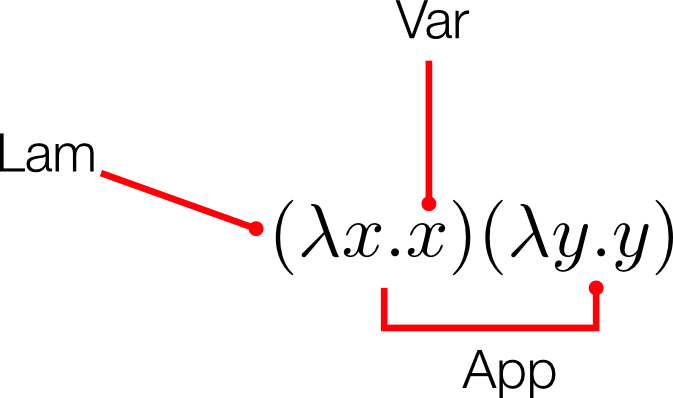
\includegraphics[width=.6\textwidth]{img/01.png}
	\caption{Structure of lambda terms}
	\label{fig:funcapp}
\end{figure}  
\end{frame}


\begin{frame}
\frametitle{Alpha Equivalence}

\section{Alpha equivalence}

We have seen the function
\begin{center}
$\lambda x.x$
\end{center}
The variable $x$ here is not semantically meaningful except in its role in that single expression. Because of this, there’s a form of equivalence between lambda terms called alpha equivalence. In other words, 
\begin{center}
$\lambda x.x$ \\

$\lambda apple.apple$\\

$\lambda orange.orange$\\
\end{center}
all mean the same thing. 
\end{frame}
\section{Beta reduction}
\begin{frame} [fragile, label = test]
    \frametitle{Beta Reduction}

When we apply a function to an argument, we 
\begin{itemize}
\item substitute the input expression for all instances of bound variables within the body of the abstraction
\item eliminate the head of the abstraction (its only purpose was to bind a variable)
\end{itemize}
This process is called beta reduction.

\end{frame}

\begin{frame} [fragile, label = test]
    \frametitle{More Beta reduction}
  
   \begin{center}
   $\lambda x.x$
   \end{center}
   \pause
   \begin{itemize}
   \item We apply the function above to 2
   \pause
   \item substitute 2 for each bound variable in the body of the function, and 
   \pause
   \item eliminate the head:
   \end{itemize}
   \begin{center}
    \pause
   $(\lambda x.x) \ 2  $ \\
   
   \hspace*{.5in}2
   \end{center}
   \pause
   The only bound variable is the single $x$, so applying this function to 2 returns 2. This function is the \textit{identity} function.

   \end{frame}

\begin{frame} [fragile, label = test]

 \frametitle{More Beta reduction}
Other Examples: 
\pause
\begin{center}
$(\lambda x.x+1)$
\end{center}
What happens if we apply this to 2?  (Try this yourself)\\
\pause
We can also apply our identity function to another lambda abstraction:
\begin{center}
$(\lambda x.x)(\lambda y.y)$
\end{center}
\pause
In this case, we substitute the entire abstraction in for $x$. We use a new syntax here, $[x := z]$, to 
indicate that $z$ will be substituted for all occurrences of $x$ (here $z$ is the 
function $(\lambda y.y)$). We reduce this application like this:
\pause
\begin{center}
$(\lambda x.x)(\lambda y.y)$ \\

$[x  := (\lambda y.y)]$\\

\hspace{.4in}$(\lambda y.y)$\\
\end{center}
Our final result is another identity function. There is no argument to apply it to, so we have nothing to reduce.
\end{frame}
\begin{frame} [fragile, label = test]
\frametitle{More Beta reduction}
Once more, but this time we’ll add another argument:
\begin{center}
$(\lambda x.x)(\lambda y.y)z$
\end{center}
\pause
Applications in the lambda calculus are left associative. That is, unless specific parentheses suggest otherwise, they associate, or group, to the left. So, it can be rewritten as:
\begin{center}
$((\lambda x.x)(\lambda y.y)) z$
\end{center}
\pause
The $\beta$-reduction is as follows:
\begin{center}
$((\lambda x.x)(\lambda y.y)) z$ \\

\hspace{.22in}$[x := ( \lambda y. y) ] $\\

\hspace{.58in}$ (\lambda y.y) z $ \\

\hspace{.58in}$[y:= z ] $\\

\hspace{1in}$z$ \\
\end{center}
\pause
We can't reduce this any further as there is nothing left to apply, and we know nothing about $z$.
\end{frame}
\section{Variables}
\begin{frame} [fragile, label = test]
    \frametitle{Variables}
     
    Variables can be 
    \begin{itemize}
        \item bound or 
        \item free 
    \end{itemize}

        as the $\lambda$-calculus assumes an infinite universe of free
    variables. They are bound to functions in an environment, then they become bound by usage in an abstraction. \\
    \pause
    For example, in the $\lambda$-expression:
    \begin{center}
    $(\lambda x. x*y)$
    \end{center}
    \pause
    x is bound by $\lambda$ over the body $x*y$, but $y$ is a free variable.When we apply this function to an argument, nothing can be done with the $y$. It remains irreducible.
    \end{frame}

    \begin{frame} [fragile, label = test]
        \frametitle{Variables contd. }
        Look at the following when we apply such a function to an argument:  
        \pause
        \begin{center}
        $(\lambda x.x*y)z$
        \end{center}
        \pause
        We apply the lambda to the argument $z$. \\
        \begin{center}
        $(\lambda x.x*y)z$ \\
        
        \hspace{.25in}$[x:=z]$ \\
        
        \hspace{.55in}$zy$  \\
        
        \end{center}
        \pause
        The head has been applied away, and there are no more heads or bound variables. Since we know nothing about $z$ or $y$, we can reduce this no further.
        \end{frame}
        \begin{frame} [fragile, label = test]
            \frametitle{Multiple Arguments }
            \section{Multiple arguments}
            Each lambda can only bind one parameter and can only accept one argument. Functions that require multiple arguments have multiple, nested heads. When you apply it once and eliminate the first (leftmost) head, the next one is applied and so on. This means that the following
            \begin{center}
            $\lambda xy.xy$
            \pause
            \end{center}
            is simply syntactic sugar for 
            \begin{center}
            $\lambda x(\lambda y.xy)$
            \end{center}
            
            \end{frame}
            
\begin{frame} [fragile, label = test]
            \frametitle{Lambda Caculus in Haskell}
           \section {Using lambda Calculus in Haskell}
           How do we write lambda expressions in Haskell? 
           \pause
           \begin{center}
           \begin{tabular}{ | c | c |  c| c|} 
             \hline
             Named &Lambda Calculus & Lambda Calculus & Result \\ 
             Function&  (maths)& (Haskell) & \\ 
            
             \hline
             $f \ x = x+1 $&( $\lambda x.x+1)$ 2 & $ (\setminus x \rightarrow  x+1)$ 2 & 3\\ 
             $f \ x \ y = x*y  $ &( $\lambda x \ y .x*y)$ 2\ 3 & $ (\setminus x \ y \rightarrow  x*y )$ 2 \ 3 & 6\\ 
            %$( $\lambda f. zipWith \ f [1 \ldots 5] [1\ldots 5]) $  $(*)$ & $ (\setminus f  \rightarrow zipWith \ f [1 \ldots 5] [1\ldots 5]))$ $(*)$  \\ 
             $f \ xs = `c`:xs$ &( $\lambda xs. `c`:xs) $  \ "at"  & $ (\setminus xs \rightarrow  `c`:xs)$  \ "at" & "cat"\\ 
             \hline
           \end{tabular}
           \end{center}
           \pause
           Lambda functions are used extensively in Haskell, notably with Higher Order Functions. 
           \end{frame}          
\begin{frame}
    \frametitle{Encoding Lambda Calculus}
    \begin{itemize}
        \item Alonzo Church is probably most well known for inventing lambda calculus, 
        \pause
        \item Church encodings were developed by Alonzo Church
        \pause
       \item Church encodings are a very interesting development arising from lambda calculus,
       \pause 
       \item Church found out that every concept in programming languages can be represented using  functions! 
       \pause
       \item Everything from boolean logic, conditional statements, numbers (natural, integer, real, complex, imaginary), and even loops (infinite loops also)!
    \end{itemize}        
            
            \end{frame}
\begin{frame}
\frametitle{Encoding Lambda Calculus.. contd. }
\begin{itemize}
    \item So how do we encode all these
    constructs using only functions?
    \pause
    \item \textbf{Idea:}  Encode the \textbf{\textit{behavior}} of values
and not their structure
\end{itemize}
\end{frame}

\begin{frame}
    \frametitle{Encoding Booleans in $\lambda$ Calculus }
    \begin{itemize}
    \item What can we do with a boolean?
    \item We can make a binary choice (\textbf{\textit{if}}  expression)
    \item A boolean is a function that, given two choices, selects one of them:
    \end{itemize}
    \begin{eqnarray*}
        TRUE = \lambda x . \lambda y.  x \\ \\
        FALSE = \lambda x . \lambda y.  y \\ \\
    \end{eqnarray*}

\end{frame}

\begin{frame}
    \frametitle{Encoding Booleans in $\lambda$ Calculus }
 So how do we encode \textbf{NOT} \\  
 \vspace{1cm}
 if we think of the structure :  \\
 \pause
 \begin{eqnarray*}
    if\  b \ then \ FALSE; \\
    else \  TRUE 
\end{eqnarray*}
 \pause
 \begin{eqnarray*}
NOT = \lambda b . b\  FALSE\  TRUE 
\end{eqnarray*}
\end{frame}


\begin{frame}
    \frametitle{Encoding Booleans in $\lambda$ Calculus }
 \begin{eqnarray*}
NOT = \lambda b . b\  FALSE\  TRUE 
\end{eqnarray*}

Let's test this  on \alert{$NOT \ TRUE$}:
\begin{eqnarray*}
    NOT = \lambda b . b\  FALSE\  TRUE \\ \\
    NOT \ \ TRUE \\ \\
    ( \lambda b . b\  FALSE\  TRUE )\  TRUE \\ \\
    (TRUE)\  FALSE\ TRUE  \\ \\
    = FALSE  \\ \\
\end{eqnarray*}
\end{frame}
\begin{frame}
    \frametitle{Encoding Booleans in $\lambda$ Calculus }
    Next, let's test this  on \alert{$NOT \ FALSE$}:
    \begin{eqnarray*}
    NOT \ \ FALSE \\ \\
    ( \lambda b . b\  FALSE\  TRUE )\  FALSE \\ \\
    (FALSE)\  FALSE\  TRUE  \\ \\
    = TRUE
    \end{eqnarray*}
\qed
\end{frame}
\begin{frame}
  
                \frametitle{Encoding Lambda Calculus.. Exercise}
                Using the techniques above, encode the following using lambda calculus:
                \begin{enumerate}
                    \item AND 
                    \item OR 
                \end{enumerate}
            \end{frame}
\begin{frame}
  
    \frametitle{Encoding Lambda Calculus..video}
        For a very good introduction to lambda calculus and encoding boolean logic 
        using lambdas, see link to Graham Hutton's video (Computerphile) 
        \href{https://youtu.be/eis11j_iGMs}{here} 
       \\ 
       \vspace{1cm}

        (You'll need to view this pdf 
        through Adobe Reader to use the link. Otherwise Google 'youtube Lambda Calculus Computerphile Graham Hutton')
     \end{frame}

\end{document}